\section{Introduction}
Once developed for the military sector, Unmanned Aerial Vehicles (UAV) are gaining popularity in private as well as commercial sector. One often-mentioned use-case is the logistics use case, particularly parcel delivery. A number of big companies such as Amazon have already announced plans to implement UAV-based home delivery systems \cite{stolaroff.2014}. It looks like in the near future UAVs might deliver parcels to your doorstep. The logistics industry hopes for positive impacts on their costs and competitiveness. The deployment of such a delivery concept is quite complex. It requires efficient path finding algorithms and an inter-vehicle communication, which is very challenging \cite{bekmezci.2013}.\\
To allow early evaluation and reduce the number of required costly flight-testing, a simulation engine is required. This paper proposes a simulation engine for multiple UAV delivery scenario based on agent-based modelling (ABM). It supports a number of depots and UAVs as well as simple change of path-planning algorithm. UAVs operate in a 3D environment with realistic building shapes. The engine does not simulate the behavior of the UAV in the aerial space itself, but allows the evaluation of spatial distribution of depots or the suitability of a path-planning algorithm. It was developed considering the use of distributed control algorithms for self-organization and swarm algorithms in the delivery use-case and allows the avoidance of a central ground control due to inter-drone communication and autonomous organization.\\
In the following section, related literature will be evaluated, followed by a detailed description of the simulation scenario (section \ref{sec:scenario}. A detailed description of the various components and frameworks used for implementation is given in section \ref{sec:model}. In section \ref{fig:algorithm} a sample implementation of a distributed algorithm based on the A* path planning algorithm \cite{hart.1968} will be presented and evaluated in the following section (section \ref{sec:evaluation}). The evaluation also contains a discussion on the simulation's performance and improvements. Finally, the conclusion outlines the paper, its limitations and future development.

\section{Related Work}
The literature on simulation engines for a UAV parcel delivery scenario is still relatively scarce. In general the researchers concentrate more on specific components or fight behavior rather than the whole delivery use case. Eric Johnson and Sebastien Fointaine developed a simulation engine for the behavior of specific hardware components of a UAV \cite{johnson.2001}. Their research focuses mainly on low-cost UAVs with limited capacities. The simulation provides high benefit for minimal effort and enables simulations with reasonable costs, taking into account the limited resources of the UAVs without accessing the UAVs actual hardware. Lu and Geng (2011) simulated the flight dynamic behavior of a UAV using Matlab/Simulink focusing on the control law of UAVs \cite{lu.2011}. They propose a Hardware-In-a-Loop (HIL) simulation based on a mathematical UAV model, that includes the characteristics of the UAV. The simulation shows very low deviations between the system and real flights and is therefore suitable to test and validate the control law designs of a UAV. \\
MultiUAV \cite{rasmussen.2003}, a very general simulation engine has been developed to simulate cooperative algorithms for finding targets. The software does not only include vehicle dynamics but also flight dynamics, based on cooperative control algorithms. The cooperative control of UAVs requires an implementation of an inter-vehicle communication which is also addressed in our research. Furthermore, an agent-based simulation engine implementing a surveillance scenario was introduced in 2005 \cite{jang.2005}. The main goal of this research was to develop efficient coordination methods for large-scale multi-agent systems. The simulation shares some similar concepts with the simulation proposed in our paper. For example, in their scenario the UAVs try to find targets without prior knowledge of the targets’ locations. The UAVs are implemented as autonomous agents that interact with each other via messages. Moreover, the notion of obstacles and bases is being used. The described sensor concept is also similar to the one used in this paper.\\
HOW ARE WE DIFFERENT?

\section{Scenario}\label{sec:scenario}
Before embarking the software model, the delivery scenario shall be explained. As mentioned in the introduction, the UAVs operate in a 3D environment representing a city. Every UAV has an assigned depot, called base-station in the application model, from which it receives items to be delivered. Every base-station is responsible for a portion of the whole city area and only contains parcels that are within this area. \\
 UAVs are assigned to one specific base-station. After receiving an item, the UAV starts moving to the item’s target destination. It scans the area and stores information on all fields it has visited on its route. If a UAV meets another UAV, they exchange information on the already explored parts of the area. There is no central unit, coordinating the UAVs. The system is based on autonomous logic of the UAVs and the inter-drone message exchange. If a field on the route contains an obstacle, the UAV will deviate from its planed route and try to find a way around the obstacle. Obstacles can have different heights and UAVs are able to fly different heights excluding different slopes. \\
After delivering the item, the UAVs fly back to the base-station to receive a new item. The limited battery power of a UAV was also taken into consideration in the simulation. If the battery reaches a certain predefined threshold, the UAV will target the next nearest base-station (not necessarily its home base) and recharge its battery.\\
In reality, this autonomous approach is especially helpful as a central ground control requires complex radio infrastructure and can fail and stop the operations of a distributor's logistics.  UAVs moving autonomously do not encounter this problem but are exposed to more complex logic which requires a proper simulation application before testing the hardware in the field.

\section{Description of the model}\label{sec:model}
The simulation has been written in Python, using the MESA \cite{masad.2015} framework for agent-based modelling. Figure \ref{fig:architecture} represents the software architecture. There are three major components: the simulation model itself, implementing the simulation environment and logic, an analytics interface for evaluating a simulation's performance and the GUI realized using a web server and allowing for easy access with a standard web-browser. The UAV as part of the simulation model, shall be described in particular in section \ref{sec:UAV}.\\
The simulation's aim is to support comparing of different decentralized path-planning algorithms by making them easily exchangeable. Predefined KPI's and an output method are used to support analyzing the performance of one's implementation. Section \ref{sec:KPI} discusses the way KPI's are defined.\\
\begin{figure}[htbp]\label{fig:architecture}
	\centering
	\includegraphics[scale=0.3]{images/architecture.png} 
	\caption{Architecture of simulation model}
\end{figure}
Figure \ref{fig:architecture} shows the architecture of the simulation model. In general, the model contains of a UI component including configurationa and GUI, the model containing the UAV, the world model and the programming logic and the data analysis component which writes out the simulation results to allow for further evaluation. 


\subsection{MESA}
MESA \cite{masad.2015} is an open source agent-based modeling framework (ABM) developed specifically for the Python programming language.  Agents are objects that have rules and states that act accordingly on every step of the simulation \cite{axtell.2000}. ABM allows to capture the path of the simulation along with the solution and allows for analysing the dynamic history \cite{axtell.2000}. ABM also allows to dynamically pause and resume the simulation at any given step and analyse the current results.\\
MESA comes with implementations of important components, such as a grid for implementing a simple 2D environment, a web-browser-based UI, a data analysis tool and an agent scheduler. Our simulation makes use of some of these components while modifying others to suit our needs. We use the data collector, the scheduler and the agent base class without modifications. The scheduler activates the agents and triggers an action. We use the RandomActivation which means that in every step the agents are activated in a random order. The DataCollector is used for collecting relevant quantitative data to support the evaluation of an algorithm.\\
To better fit our needs, we modified the MESA grid, visualization elements and the visualization server. In the following section we describe what we changed and explain the reasons behind the modifications.
The MESA grid is "a simple list-of lists" \footnote{|url{ttp://mesa.readthedocs.io/en/latest/apis/space.html}}. Each entry in such a grid has to be an agent. Since we wanted to perform our simulation on a larger scale, i.e. on a 500 x 500 grid, we had to place a lot of obstacles to come up with a realistic simulation environment. With such a huge amount of obstacles we experienced severe performance issues. The reasons behind this is the standard visualization element that is used to render the grid. The visualization element iterates over all registered agents and renders them in the GUI. As a result we decided to not consider obstacles as agents. Instead, we introduced our own grid, which is a matrix, that only contains numeric values. Each value represents either an obstacle, a base station or "nothing". 
 
\subsection{User Interface: Configuration and GUI}
The user interface consists of two parts: The file \textit{config.ini} to change the simulation scenario and a web server responsible for rendering the GUI and delivering it through a web browser.\\
The configuration file is being parsed at the startup of the simulation engine and contains all the required settings for the simulation to work properly. It contains crucial information that have a high impact on an algorithm's performance and makes it easy to set up different scenarios, e.g. one might consider testing the results using different number of UAVs per depot or more or less depots itself.
Furthermore the impact of different battery capacity (in steps) can easily be simulated. A higher sensor range can be beneficial for an algorithm's performance but should be chosen realistically according to the model.\\
As mentioned earlier, the GUI is implemented using a web server. For the GUI to properly function, two image files are required. One contains the map as the user is supposed to see it. The other one stores information on obstacles and their respective heights using color codes. White means that there is no obstacle and other colors represent different altitude levels. An obstacle is any static object (such as trees or buildings etc.) that obstructs the movement of the UAV. The file will be parsed on start-up and the information stored in the model.  Depots are placed on obstacles. %Compare figure  \ref{fig:gui} for an overview of the GUI.
%\begin{figure}[htbp]\label{fig:gui}
%	\centering
%	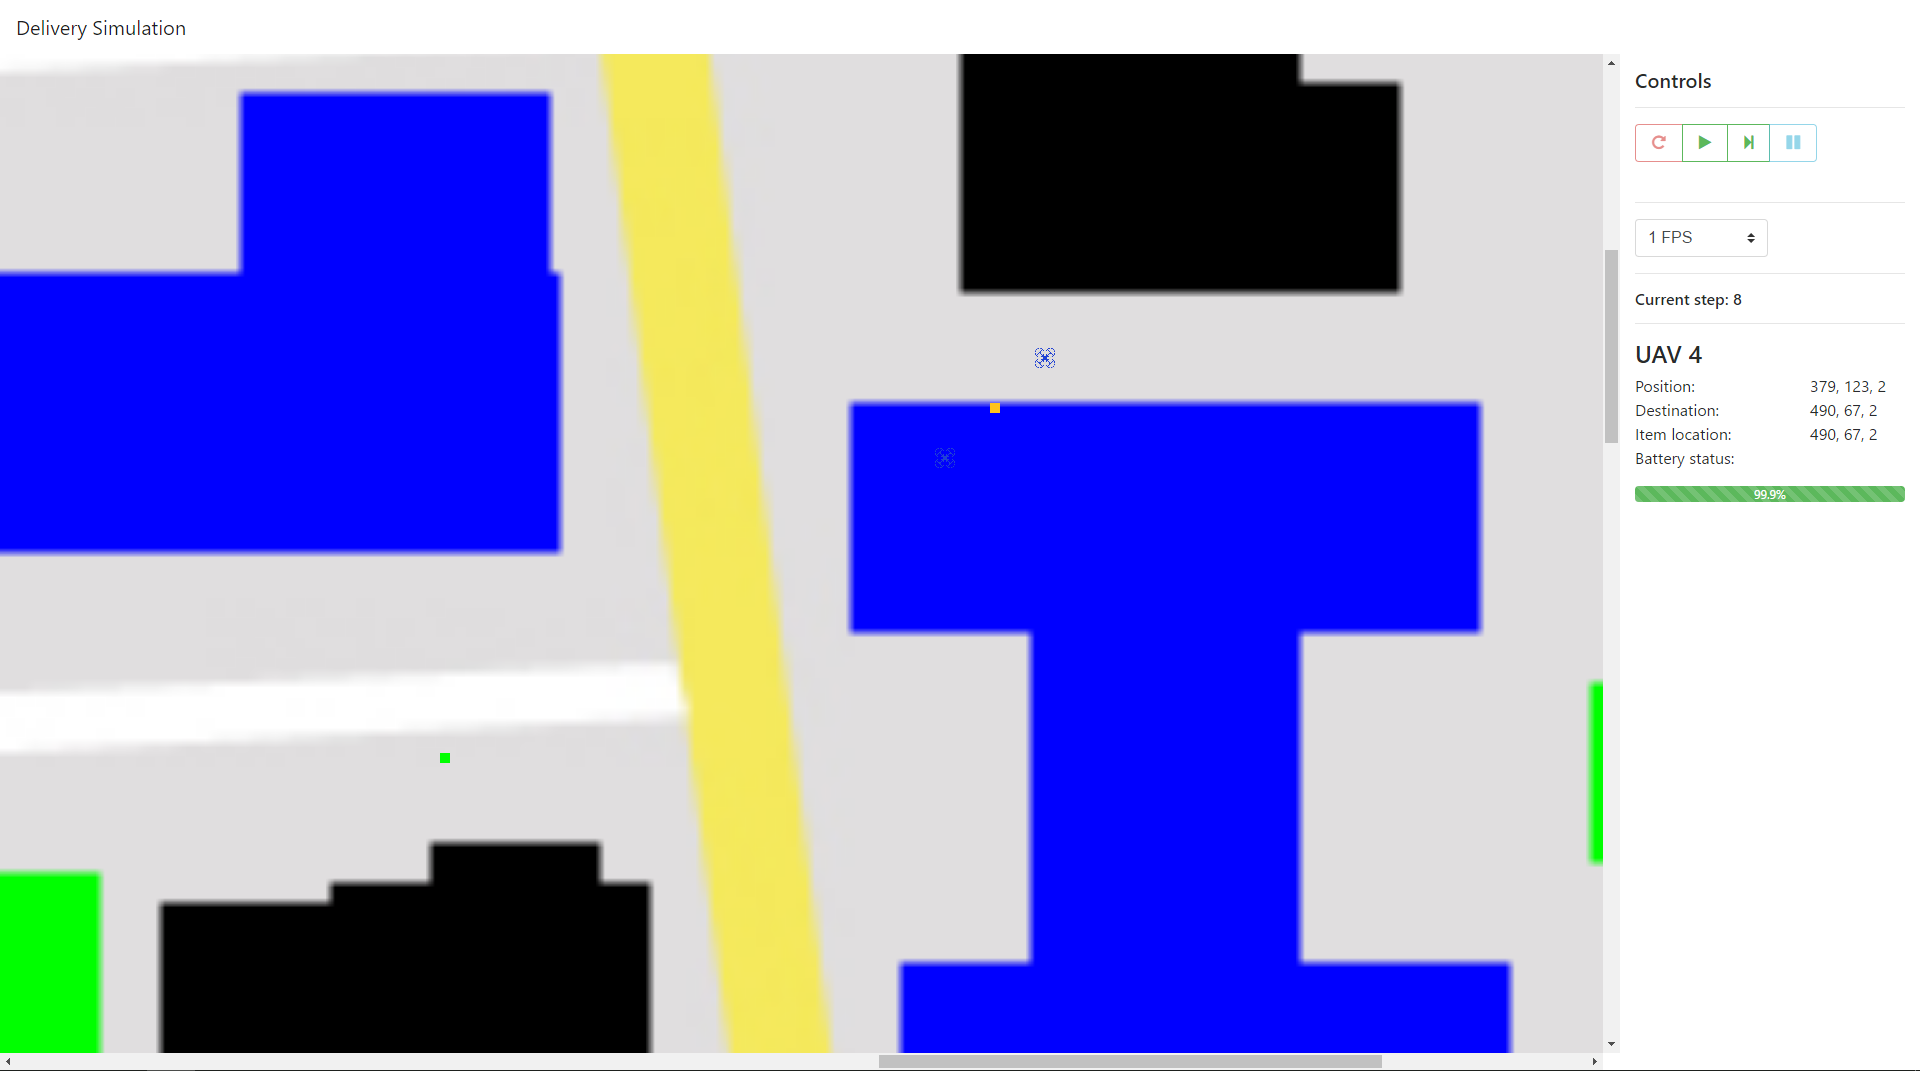
\includegraphics[scale=0.4]{images/gui}
%	\caption{The GUI of the simulation engine}
%\end{figure}
The GUI allows for starting, pausing and resetting the simulation and shows the movement of UAVs in the space. It is implemented in a 2D fashion although internally the model calculates with 3-dimensional coordinates. The image's color codes for obstacles are used to represent the different altitudes. For now, the simulation tool supports 5 different height levels but one can easily modify the parser and define more colors for more altitude levels.
To be able to see more detailed information on each agent (UAV, base station and item), one can click on the visual representation of the agent. The click activates a detail view. The detail view for UAV can be seen in figure \ref{fig:uav_detail}.

	\begin{figure}[htbp]\label{fig:uav_detail}
		\centering
		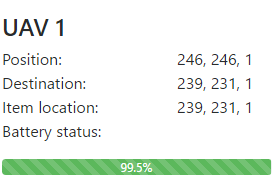
\includegraphics[scale=0.5]{images/uav_detail.png}
		\caption{Detailed view of UAV}
	\end{figure}


\subsection{Agents}\label{sec:UAV}
The most important agent of a UAV simulation is the UAV itself. We developed a realistic simulation representing the required components and behavior and omitted not required components to cover the delivery scenario. The simulated UAV has the following components:
	\begin{itemize}
			\item \textbf{Battery}: The battery has a limited battery life that decreases on each step. When the battery reaches a certain threshold (configurable), the UAV will fly to the nearest depot to recharge.
					\item \textbf{CargoBay:} The cargoBay represents the UAV's storage unit which can store one item.
		\item \textbf{FlightController:} This component contains the path-finding/route-planning algoritm. It represents a navigation unit. Multiple algorithms could be implemented, compare section \ref{sec:algorithm} for an example. The algorithm uses the sensor to identify its neighboring fields at any step. Additionally it stores a perceived world which holds all fields that are already explored. The component can access all information from the other component and the UAV itself. On every step, the UAV calls the method "make\textunderscore step()" which has to be implemented in case of changing the algorithm.
		\item \textbf{CommunicationModule:} If the sensor found another UAV in the sensor's radius, this component will communicate with the other UAV and exchange grid information. Exchange of information on previously-unknown terrain helps when a UAV has to deliver an item to a new area of the map. This allows for precomputing optimal routes before exploring the actual area.
		\item \textbf{Sensor:} Scanning the grid for obstacles and other agents. This component is the interface to the model
	\end{itemize}

UAVs do not communicate with a central entity such as a control server organizing the flight traffic. They communicate with each other if they are in sensor range and only rely on their own sensor.
To optimize performance for the exchange of grids, the UAVs only store a dictionary containing their perceived world rather than a full matrix implemented in MESA's grid.
There is one dictionary for each height level, mapping coordinates to information whether there is an obstacle on that field or not.  
\\
The second agent in the simulation is the BaseStation. In the real world, this is the depot of a logistics company. It assigns orders to UAVs and hands items over to them. Depots are responsible for all items in a part of the map and for a subset of all drones. Also, they contain chargers for UAVs whose battery reached a low level. In the configuration, one can set how many depots are supposed to be on the map by specifying the number of fields the depot is responsible for (its delivery area). Depots are located as close to the center of their area as possible, but only on obstacles (on buildings). Items that are picked up from a depot can have different priorities in order to make the simulation more realistic. For example, items with high priority can be important and immediately required medical equipment or parcels for which a customer paid a higher fee to receive it faster.



\subsection{Analytics}\label{sec:KPI}
During a run, data and results are being generated. To allow for the evaluation of a path finding algorithm
For evaluating the delivery scenario, we identified the following KPI's:
\begin{itemize}
	\item \textbf{Average walk length:} Describes the average number of steps taken for an item to be delivered. 
	\item \textbf{Average walk length divided by initial distance:} This data point is a ratio calculated by dividing the average number of steps taken by the initial distance from base station to an item's destination. The initial distances are calculated as euclidean distances. Example: A value of 2 means that the average walk length is 2 times the initial distances.
	\item \textbf{Standard deviation of average walk lengths:} Represents the standard deviation of all walk lengths to get a better insight into the data additional to the average walk length.
	\item \textbf{Items delivered per UAV:} Items delivered divided by number of UAV's.
	\item \textbf{Average lifetime of item:} Calculation of the average lifetime of items by aggregating all item's lifetimes, divided by number of items. Lifetime is defined as the time from being available for delivery at the depot to the actual delivery at the item's destination.
\end{itemize}

The results are step-wise written out into a CSV file during the simulation and can for example be imported into a spreadsheet software or more sophisticated tools like R or any other application to run statistical analysis of the KPI's. Technically, this is realized by using MESA's DataCollector class. This allows for easy definition of values be calculated every step and export them to a CSV file. The KPI's can easily be extended or modified in the source code.

\section{Implementation of a sample algorithm: A Star}\label{sec:algorithm}
WORK IN PROGRESS
\begin{itemize}
	\item Describe algorithm based on \cite{hart.1968}
	\item Describe how we implemented the search
	\item The implementation was tested in four scenarios on a 500x500 map with five altitude levels: two scenarios with 2 BaseStations and 5 and 10 UAV per BaseStation, respectively. The two other scenarios involve 10 BaseStations and 5/10 UAVs as well. These scenarios simulate different density of depots in the city with varying numbers of UAVs. We expected that a very big number of UAVs leads to a slow-down in simulation due to expensive inter-drone communication and exchange of explored areas. A higher density of UAVs should lead to faster exploration of the area, more communication and thus allow for less computation steps of the algorithm we implemented. After a certain number of steps, the required steps for delivering should decrease as UAVs gained knowledge of their area and are able to calculate best routes. Every scenario was run for 5000 steps. If one considers one step as one simulated second, this means the simulation runs for almost 90 minutes.

\end{itemize}
\section{Evaluation}\label{sec:evaluation}
The simulation engine presented in this paper allows for a simple evaluation of a path planning algorithm in a 3-dimensional space. Also it helps to iexpose traditional algorithms to a swarm optimization problem as UAVs exchange their grid whenever they come close enough to each other.\\
 A bottleneck is the calculation performance. On a mid-2015 Apple Macbook Pro with a i5 Dual core processor, the calculation of 5000 steps (run without GUI) still takes a very long time. This is due to the fact that the implementation of the MESA grid used in the model is not performance-optimized. Also, the exchange of the grid is a complex task. It was tried to optimize performance by using dictionaries for the UAV's perceived world rather than storing a complete matrix. The model's internal grid also has been modified to just store numerical values for obstacles (1+ altitude), baseStations/depots (-1) or 0 for no content.

\section{Conclusion}\label{sec:conclusion}
This paper presented a new simulation engine specifically developed for the delivery use-case with autonomous UAV not being controlled by a central control server. Delivery of items will be relevant in the near future and a simulation engine is required to test for different scenarios, such as different numbers of depots or rural against urban regions. The engine supports multiple depots and UAVs, communication between UAV and different altitude levels for testing. It is based on the MESA modeling framework whereas many adjustments for performance have been implemented. The GUI allows for visual evaluation of the simulation's progress and the CSV output helps analyzing the final scenario results. The simulation of a battery helps to understand how far a destination should be from a depot and thus how many depots are required. \\
The engine does not support UAVs carrying more than one item nor changing the input file for the map. Currently it comes with an example map but in the future this should be exchangeable. 



